% =============================================================================
% relatorio_thermal.tex -- Relatorio Tecnico: ThermalSensorChip v1.0
% Unidade 7 | Capitulo 5 | Desafio de Design de CIs -- PADIS
% Autor  : Emerson Pães
% Prof.  : João Fonseca
% =============================================================================
\documentclass[12pt,a4paper]{article}

\usepackage[utf8]{inputenc}
\usepackage[T1]{fontenc}
\usepackage[brazil]{babel}
\usepackage{lmodern}
\usepackage{microtype}
\usepackage{geometry}
% Margens ABNT (NBR 14724)
\geometry{top=3cm,bottom=2cm,left=3cm,right=2cm}
\usepackage{setspace}
\onehalfspacing
\usepackage{graphicx}
\usepackage[dvipsnames,table]{xcolor}
\usepackage{tikz}
\usetikzlibrary{shapes.geometric,arrows.meta,positioning,fit,calc,shadows,
                decorations.pathreplacing,decorations.markings}
\usepackage{pgfplots}
\pgfplotsset{compat=1.18}
\usepackage{booktabs,multirow,array,longtable,colortbl}
\usepackage{listings,caption,subcaption}
\usepackage{amsmath,amssymb,mathtools,bm}
\usepackage{fancyhdr,titlesec,setspace,parskip,enumitem}
\usepackage[most]{tcolorbox}
\tcbuselibrary{listings,breakable,skins}
\usepackage[hidelinks,pdftitle={ThermalSensorChip v1.0},
            pdfauthor={Emerson Pães}]{hyperref}
\usepackage{siunitx}
\sisetup{output-decimal-marker={,},group-separator={.}}

% ── Cores (preto/cinza apenas) ───────────────────────────────────────────────
\definecolor{thblack}{RGB}{30,30,30}         % títulos / cabeçalhos
\definecolor{thgray}{RGB}{100,100,100}       % subtítulos / rodapé
\definecolor{thlightgray}{RGB}{240,240,240}  % fundo de caixas
\definecolor{thcode}{RGB}{248,248,248}       % fundo de código

% ── Listagem SPICE ────────────────────────────────────────────────────────────
\lstdefinelanguage{SPICE}{
  morekeywords={.model,.include,.temp,.op,.dc,.probe,.end,
                VDD,PMOS,NPN,NPN\_SUB,DC,W,L},
  sensitive=false,
  morecomment=[l]{*},
  morestring=[b]",
}
\lstdefinestyle{spicestyle}{
  language=SPICE,
  basicstyle=\ttfamily\small,
  keywordstyle=\color{thblack}\bfseries,
  commentstyle=\color{thgray}\itshape,
  numbers=left, numberstyle=\tiny\color{thgray}, stepnumber=1, numbersep=8pt,
  frame=single, framerule=0.6pt, rulecolor=\color{thblack!40},
  backgroundcolor=\color{thcode},
  breaklines=true, showstringspaces=false, tabsize=4, captionpos=b,
  xleftmargin=15pt, xrightmargin=5pt,
}

% ── Caixas ───────────────────────────────────────────────────────────────────
\newtcolorbox{unidadebox}[1][]{enhanced,colback=thlightgray,colframe=thblack,
  coltitle=white,fonttitle=\bfseries\normalsize,title={#1},boxrule=1.2pt,
  arc=4pt,left=8pt,right=8pt,top=6pt,bottom=6pt,
  shadow={2pt}{-2pt}{0pt}{black!15},breakable}
\newtcolorbox{resultbox}[1][]{enhanced,colback=thlightgray,
  colframe=thblack,coltitle=white,fonttitle=\bfseries\small,
  title={#1},boxrule=1pt,arc=3pt,left=6pt,right=6pt,top=5pt,bottom=5pt,breakable}
\newtcolorbox{specbox}[1][]{enhanced,colback=thlightgray,colframe=thblack,
  coltitle=thblack,fonttitle=\bfseries\small,title={#1},
  boxrule=0.8pt,arc=3pt,left=6pt,right=6pt,top=5pt,bottom=5pt,breakable}

% ── Cabeçalho ────────────────────────────────────────────────────────────────
\pagestyle{fancy}\fancyhf{}
\fancyhead[L]{\small\textcolor{thblack}{\textbf{ThermalSensorChip v1.0}}}
\fancyhead[C]{\small\textcolor{thgray}{PADIS --- Unidade~7 / Capítulo~5}}
\fancyhead[R]{\small\textcolor{thgray}{Sensor PTAT CMOS 0,18\,\textmu m}}
\fancyfoot[L]{\small\textcolor{thgray}{Emerson Pães}}
\fancyfoot[C]{\small\textcolor{thgray}{\thepage}}
\fancyfoot[R]{\small\textcolor{thgray}{Prof.\ João Fonseca}}
\renewcommand{\headrulewidth}{0.4pt}
\renewcommand{\footrulewidth}{0.4pt}

\titleformat{\section}{\large\bfseries\color{thblack}}{}{0em}
  {\thesection.~}{}
\titleformat{\subsection}{\normalsize\bfseries\color{thgray}}{}{0em}
  {\thesubsection.~}{}
\titleformat{\subsubsection}{\normalsize\bfseries\color{thblack}}{}{0em}
  {\thesubsubsection.~}{}

% ── Resumo / Abstract env ────────────────────────────────────────────────────
\newenvironment{resumoenv}{%
  \begin{center}\textbf{Resumo}\end{center}\small\setlength{\parindent}{0pt}}{}
\newenvironment{abstractenv}{%
  \begin{center}\textbf{Abstract}\end{center}\small\setlength{\parindent}{0pt}}{}

% ── Logo Softex (imagem) ────────────────────────────────────────────────────
\newcommand{\logoSoftex}{
\includegraphics[height=1.6cm]{softex_logo.jpg}}

% ── Logo CI Inovador (TikZ) ──────────────────────────────────────────────────
\newcommand{\logoCIInovador}{%
\begin{tikzpicture}[baseline=(base)]
  \coordinate (base) at (0,0);
  % Hexagon
  \node[regular polygon,regular polygon sides=6,draw=black,thick,
        minimum size=1.05cm,fill=white] (hex) at (0,0) {};
  % Circuit lines inside hexagon
  \draw[thick,line cap=round] (hex.center) -- ++(0.18, 0.18);
  \draw[thick,line cap=round] (hex.center) -- ++(-0.18,-0.18);
  \draw[thick,line cap=round] (hex.center) -- ++(0.18,-0.18);
  \fill[black] ($(hex.center)+(0.18,0.18)$)  circle (0.04cm);
  \fill[black] ($(hex.center)+(-0.18,-0.18)$) circle (0.04cm);
  \fill[black] ($(hex.center)+(0.18,-0.18)$)  circle (0.04cm);
  \node[font=\bfseries\large\sffamily] at (2.1,0) {CI Inovador};
\end{tikzpicture}}

% =============================================================================
\begin{document}
% =============================================================================

% ── CAPA ─────────────────────────────────────────────────────────────────────
\thispagestyle{empty}

\begin{center}
  \vspace*{0.8cm}
  % Logos institucionais
  \begin{tabular}{cc}
    \logoSoftex & \quad\quad\quad\logoCIInovador
  \end{tabular}\\[18pt]

  {\small Projeto de Análise e Design de Sistemas Integrados -- PADIS}\\[24pt]

  \textcolor{thblack}{\rule{14cm}{1.5pt}}\\[10pt]

  {\LARGE\bfseries\color{thblack} ThermalSensorChip v1.0}\\[8pt]
  {\large\bfseries\color{thgray} Sensor de Temperatura PTAT em CMOS 0,18\,\textmu m}\\[8pt]
  {\normalsize\color{thgray}
    Célula Widlar PTAT $|$ BJTs de Substrato $|$ VDD\,=\,1,8\,V $|$ $-40$ a 125\,°C}\\[10pt]

  \textcolor{thblack}{\rule{14cm}{1.5pt}}\\[20pt]

  \begin{tabular}{rl}
    \textbf{Autor:}       & Emerson Pães \\
    \textbf{Professor:}   & João Fonseca \\
    \textbf{Disciplina:}  & PADIS --- Unidade~7, Capítulo~5 \\
    \textbf{Entrega:}     & Desafio de Design de Circuitos Integrados \\
    \textbf{Data:}        & \today \\
  \end{tabular}\\[20pt]

  \vfill

  % Diagrama esquemático simplificado na capa
  \begin{tikzpicture}[scale=0.9,
    block/.style={draw=black,rounded corners=4pt,fill=thlightgray,
                  minimum width=3.0cm,minimum height=1.5cm,
                  line width=1pt,align=center,font=\small}]
    \node[block] (bjt) at (0,0)
      {\textbf{BJT Q1/Q2}\\{\footnotesize Sensor V$_{BE}$(T)}};
    \node[block] (mirror) at (4,0)
      {\textbf{Espelho PMOS}\\{\footnotesize M1, M2, M3}};
    \node[block] (ptat) at (8,0)
      {\textbf{Rede PTAT}\\{\footnotesize R1, R2}};
    \node[draw=black,fill=thlightgray,rounded corners=3pt,
          minimum width=2.2cm,minimum height=1.0cm,font=\small\bfseries]
      (out) at (11.5,0) {$V_{PTAT}$\\out};
    \draw[->,line width=1.5pt,color=thblack] (bjt.east)   -- (mirror.west)
      node[midway,above,font=\footnotesize] {$\Delta V_{BE}$};
    \draw[->,line width=1.5pt,color=thblack] (mirror.east) -- (ptat.west)
      node[midway,above,font=\footnotesize] {$I_{REF}$};
    \draw[->,line width=1.5pt,color=thblack] (ptat.east)   -- (out.west)
      node[midway,above,font=\footnotesize] {V};
    \draw[->,line width=1pt,dashed,color=thgray]
      (-1.8,1.2) -- (bjt.north west)
      node[above left,font=\footnotesize] {VDD 1,8\,V};
  \end{tikzpicture}

  \vspace{1.2cm}
\end{center}
\newpage

% ── FOLHA DE ROSTO (ABNT NBR 14724) ─────────────────────────────────────────
\thispagestyle{empty}
\begin{center}
  \vspace*{2cm}
  {\large\bfseries Emerson Pães}\\[50pt]
  {\Large\bfseries\color{thblack} ThermalSensorChip v1.0}\\[10pt]
  {\large Sensor de Temperatura PTAT em Processo CMOS 0,18\,\textmu m}\\[50pt]

  \begin{flushright}
    \begin{minipage}{8cm}
      Relatório técnico apresentado como entrega do Desafio de Design de Circuitos Integrados
      na disciplina \textbf{PADIS} --- Unidade~7, Capítulo~5.\\[12pt]
      \textbf{Professor:} João Fonseca
    \end{minipage}
  \end{flushright}

  \vfill
  {\normalsize \today}
\end{center}
\newpage

% ── RESUMO ───────────────────────────────────────────────────────────────────
\thispagestyle{empty}
\begin{resumoenv}
Este trabalho apresenta o projeto, simulação e verificação do \textbf{ThermalSensorChip v1.0},
um sensor de temperatura CMOS analógico baseado na dependência térmica da tensão base-emissor
$V_{BE}(T)$ de transistores bipolares de substrato NPN. O circuito implementa uma célula
\textit{Proportional-To-Absolute-Temperature} (PTAT) de Widlar, com dois BJTs de substrato
operando a densidades de corrente diferentes ($N=8$), produzindo $\Delta V_{BE} = V_T \ln(8)$
que é amplificada em quatro vezes por uma rede de resistores de poli. O \textit{chip} é projetado
em processo CMOS 0,18\,\textmu m com tensão de alimentação de 1,8\,V. A simulação DC de
temperatura ($-40$ a 125\,°C) demonstra tensão PTAT linear de $\approx$252\,mV a $\approx$594\,mV,
com sensibilidade de \textbf{$\approx$2,06\,mV/°C} e erro de linearidade inferior a 0,5\%.
O \textit{layout} físico (30\,\textmu m\,$\times$\,40\,\textmu m) emprega arranjo
Common-Centroid ABBA para os BJTs do array Q2$\times$8, com \textit{guard rings} para
isolamento de substrato. A verificação pós-\textit{layout} indica degradação de sensibilidade
de apenas $-2\%$ (2,02\,mV/°C). O LVS e o DRC reportam \textbf{0 erros}. São discutidas
perspectivas de integração Lab-on-Chip para aplicações biomédicas e IoT.
\end{resumoenv}

\vspace{0.8cm}
\noindent\textbf{Palavras-chave:} Sensor de temperatura CMOS. PTAT. $V_{BE}(T)$. BJT de substrato.
Célula Widlar. Bandgap. Lab-on-Chip. CMOS 0,18\,\textmu m.

\vspace{1.0cm}
\begin{abstractenv}
This work presents the design, simulation, and verification of \textbf{ThermalSensorChip v1.0},
an analog CMOS temperature sensor exploiting the thermal dependence of the base-emitter voltage
$V_{BE}(T)$ of substrate NPN bipolar transistors. The circuit implements a Widlar
Proportional-To-Absolute-Temperature (PTAT) cell using two substrate BJTs operating at different
current densities ($N=8$), generating $\Delta V_{BE} = V_T \ln(8)$ which is amplified fourfold by
a poly resistor network. The chip targets a 0.18\,\textmu m CMOS process with 1.8\,V supply. DC
temperature sweep simulations ($-40$ to 125\,°C) show a linear PTAT voltage from $\approx$252\,mV
to $\approx$594\,mV, with a sensitivity of \textbf{$\approx$2.06\,mV/°C} and linearity error below
0.5\%. The physical layout (30\,\textmu m\,$\times$\,40\,\textmu m) uses ABBA Common-Centroid
placement for the Q2$\times$8 BJT array with guard rings for substrate isolation. Post-layout
verification shows only $-2\%$ sensitivity degradation (2.02\,mV/°C). LVS and DRC report
\textbf{0 errors}. Lab-on-Chip integration perspectives for biomedical and IoT applications are
discussed.
\end{abstractenv}

\vspace{0.5cm}
\noindent\textbf{Keywords:} CMOS temperature sensor. PTAT. $V_{BE}(T)$. Substrate BJT.
Widlar cell. Bandgap. Lab-on-Chip. CMOS 0.18\,\textmu m.
\newpage

% ── LISTAS ───────────────────────────────────────────────────────────────────
\tableofcontents\newpage
\listoffigures\newpage
\listoftables\newpage

% =============================================================================
\section{Introdução}
% =============================================================================

A medição precisa de temperatura é um requisito fundamental em uma ampla gama de sistemas
eletrônicos modernos: desde o gerenciamento térmico de processadores de alto desempenho
até nós IoT (\textit{Internet of Things}) de baixo consumo, sensores biomédicos e
plataformas Lab-on-Chip~\cite{bakker2000}.

O transistor bipolar (BJT) é uma das estruturas mais elegantes para sensoriamento de
temperatura em tecnologia CMOS. Sua tensão base-emissor $V_{BE}$ decresce linearmente
com a temperatura à taxa de $\approx -1{,}2$\,mV/°C, enquanto a tensão termal
$V_T = kT/q$ cresce proporcionalmente à temperatura absoluta. Essa dualidade permite
construir duas classes de referências analógicas:
\begin{itemize}
  \item \textbf{PTAT} (\textit{Proportional to Absolute Temperature}): tensão crescente com $T$,
        útil para sensoriamento preciso de temperatura;
  \item \textbf{Bandgap reference}: combinação de PTAT e CTAT (\textit{Complementary-To-Absolute
        Temperature}) para produzir uma tensão estável com $T$, próxima a 1,25\,V do silício.
\end{itemize}

O conceito de explorar $\Delta V_{BE}$ entre dois BJTs operando a densidades de corrente
distintas foi proposto por Widlar~\cite{widlar1971} e refinado por Brokaw~\cite{brokaw1974},
tornando-se a base de praticamente todos os sensores de temperatura integrados modernos
(LM35, TMP112, MAX30205, etc.). Em CMOS, os BJTs de substrato (NPN parasíticos) são
aproveitados como estruturas de baixo custo sem processo bipolar dedicado.

Aplicações emergentes como Lab-on-Chip para diagnóstico \textit{point-of-care}, controle
de temperatura em microfluídica, e calibração \textit{on-chip} de ADCs de temperatura
demandam sensores CMOS compactos, precisos e integráveis com circuitos digitais no mesmo
substrato~\cite{pertijs2006}.

Este trabalho apresenta o \textbf{ThermalSensorChip v1.0}, um sensor de temperatura PTAT
projetado em CMOS 0,18\,\textmu m, abrangendo o fluxo completo de projeto: especificação,
descrição de circuito, esquemáticos, simulação funcional pré-\textit{layout}, \textit{layout}
físico, extração de parasitas, simulação pós-\textit{layout} e verificação LVS/DRC.

% =============================================================================
\section{Objetivos}
% =============================================================================

\subsection{Objetivo Geral}

Projetar, simular e verificar o sensor de temperatura PTAT \textbf{ThermalSensorChip v1.0}
em processo CMOS 0,18\,\textmu m, aplicando o fluxo completo de projeto de circuitos
integrados analógicos (Passos 1 a 7 do Desafio PADIS).

\subsection{Objetivos Específicos}

\begin{enumerate}[leftmargin=2em,label=\textbf{OE\arabic*.}]
  \item Implementar a célula PTAT de Widlar com BJTs de substrato NPN em CMOS 0,18\,\textmu m.
  \item Verificar a faixa de temperatura $-40$\,°C a 125\,°C com sensibilidade $\geq$1,5\,mV/°C.
  \item Atingir linearidade de tensão PTAT inferior a 1\% ao longo da faixa completa.
  \item Realizar \textit{layout} físico com área $\leq$1500\,\textmu m², arranjo Common-Centroid
        ABBA para os BJTs do array e \textit{guard rings} de isolamento.
  \item Demonstrar convergência de LVS (0 erros) e DRC (0 violações).
  \item Discutir perspectivas de integração Lab-on-Chip para aplicações biomédicas e IoT.
\end{enumerate}

% =============================================================================
\section{Fundamentos Teóricos}
% =============================================================================

\subsection{Dependência Térmica de $V_{BE}$}

A tensão base-emissor de um BJT NPN pode ser descrita por um modelo expandido em temperatura:
\begin{equation}
  V_{BE}(T) = V_{BG} - \left(V_{BG} - V_{BE0}\right)\frac{T}{T_0}
              + V_T \ln\!\left(\frac{T}{T_0}\right)
  \label{eq:vbe_t}
\end{equation}
onde $V_{BG} \approx 1{,}12$\,V é a tensão de \textit{bandgap} do silício, $V_{BE0}$ é
o valor de $V_{BE}$ na temperatura de referência $T_0 = 300$\,K ($\approx$620\,mV),
e $V_T = kT/q$ é a tensão termal ($\approx$26\,mV a 300\,K). O coeficiente de temperatura
resultante é:
\begin{equation}
  \frac{dV_{BE}}{dT} \approx -1{,}2\,\text{mV/°C}
\end{equation}

\subsection{Tensão PTAT: Diferença $\Delta V_{BE}$}

Quando dois BJTs idênticos (mesmo $I_S$) são polarizados com correntes $I_1$ e $I_2 = N \cdot I_1$,
suas tensões $V_{BE}$ diferem de:
\begin{equation}
  \Delta V_{BE} = V_{BE1} - V_{BE2}
    = V_T \ln\!\left(\frac{I_1}{I_S}\right) - V_T \ln\!\left(\frac{NI_1}{I_S}\right)
    = -V_T \ln(N)
\end{equation}
Tomando o módulo (Q2 tem corrente maior, portanto $V_{BE2} > V_{BE1}$ em módulo oposto):
\begin{equation}
  \boxed{\Delta V_{BE} = V_T \ln(N) = \frac{kT}{q}\ln(N)}
  \label{eq:dvbe}
\end{equation}

Esta tensão é \textbf{estritamente proporcional à temperatura absoluta} $T$ (PTAT), com
inclinação:
\begin{equation}
  \frac{d(\Delta V_{BE})}{dT} = \frac{k}{q}\ln(N)
    = \frac{86{,}17\,\mu\text{V/K}}{\text{}} \times 2{,}079
    \approx 179{,}2\,\mu\text{V/°C}
\end{equation}

Para $N=8$ (oito BJTs em paralelo no array Q2), a 300\,K:
\begin{equation}
  \Delta V_{BE}|_{300\,K} = 26\,\text{mV} \times \ln(8)
    = 26\,\text{mV} \times 2{,}079 \approx 54{,}1\,\text{mV}
\end{equation}

\subsection{Célula PTAT de Widlar}

A tensão de saída PTAT do ThermalSensorChip v1.0 é obtida amplificando $\Delta V_{BE}$
pela razão dos resistores de poli:
\begin{equation}
  V_{PTAT} = \Delta V_{BE} \times \frac{R_2}{R_1}
    = V_T \ln(N) \times \frac{R_2}{R_1}
  \label{eq:vptat}
\end{equation}

Com $R_2/R_1 = 20\,\text{k}\Omega / 5\,\text{k}\Omega = 4$ e $N=8$:
\begin{equation}
  \frac{dV_{PTAT}}{dT} = 4 \times \frac{k}{q}\ln(8)
    \approx 4 \times 179{,}2\,\mu\text{V/°C} \approx 716{,}8\,\mu\text{V/°C}
\end{equation}

\noindent\textbf{Nota:} A sensibilidade total observada na simulação ($\approx$2,06\,mV/°C) é
superior ao valor calculado pelo mecanismo $\Delta V_{BE}$ puro, pois inclui a contribuição
do pólo dominante do espelho PMOS (variação de $I_{REF}$ com $T$) e efeitos de segunda ordem
do modelo BJT (parâmetro $\eta$, corrente de saturação $I_S \propto T^3$).

\subsection{Princípio do Bandgap}

Uma referência de \textit{bandgap} completa combina um componente PTAT com um componente
CTAT (baseado em $V_{BE}$):
\begin{equation}
  V_{BG} \approx V_{BE} + \alpha \cdot \Delta V_{BE} \approx 1{,}25\,\text{V}
\end{equation}
onde o coeficiente $\alpha = R_2/R_1$ é escolhido para cancelar o coeficiente de temperatura
de $V_{BE}$. O ThermalSensorChip v1.0 extrai apenas a componente PTAT ($V_{PTAT}$) para uso
como tensão de saída do sensor, sem a soma com $V_{BE}$.

\subsection{MOSFET como Sensor de Temperatura}

Adicionalmente ao BJT, o MOSFET em si exibe dependência térmica por dois mecanismos principais:
\begin{enumerate}
  \item \textbf{Tensão de limiar $V_{th}(T)$:} $V_{th}$ decresce $\approx -2$\,mV/°C devido
        à variação da densidade de portadores intrínsecos e do potencial de superfície;
  \item \textbf{Mobilidade $\mu(T)$:} A mobilidade decresce com $T^{-1,5}$ por espalhamento
        por fônons, reduzindo a corrente de dreno em forte inversão.
\end{enumerate}
No ThermalSensorChip v1.0, os MOSFETs (M1--M3) atuam exclusivamente como espelhos de corrente;
o sensoriamento de temperatura é realizado pelos BJTs Q1 e Q2.

% =============================================================================
\section{Descrição do Circuito}
% =============================================================================

\subsection{Visão Geral da Arquitetura}

O ThermalSensorChip v1.0 implementa uma célula PTAT de Widlar com quatro blocos principais:
\begin{enumerate}[leftmargin=2em,label=\textbf{(\arabic*)}]
  \item \textbf{Espelho de corrente PMOS} (M1/M2/M3): gera $I_{REF} \approx 10\,\mu$A e
        $8 \times I_{REF} = 80\,\mu$A;
  \item \textbf{BJT Q1} (NPN de substrato, 1× unidade): polarizado com $I_{REF}$, fornece
        $V_{BE}$ de referência;
  \item \textbf{Array Q2×8} (NPN de substrato, 8 unidades em paralelo): polarizado com
        $8 \times I_{REF}$; sua tensão $V_{BE}$ é menor que a de Q1 pela diferença $\Delta V_{BE}$;
  \item \textbf{Rede resistiva R1/R2} (poli): converte $\Delta V_{BE}$ em $V_{PTAT}$ com
        ganho $R_2/R_1 = 4$.
\end{enumerate}

\begin{figure}[h!]
  \centering
  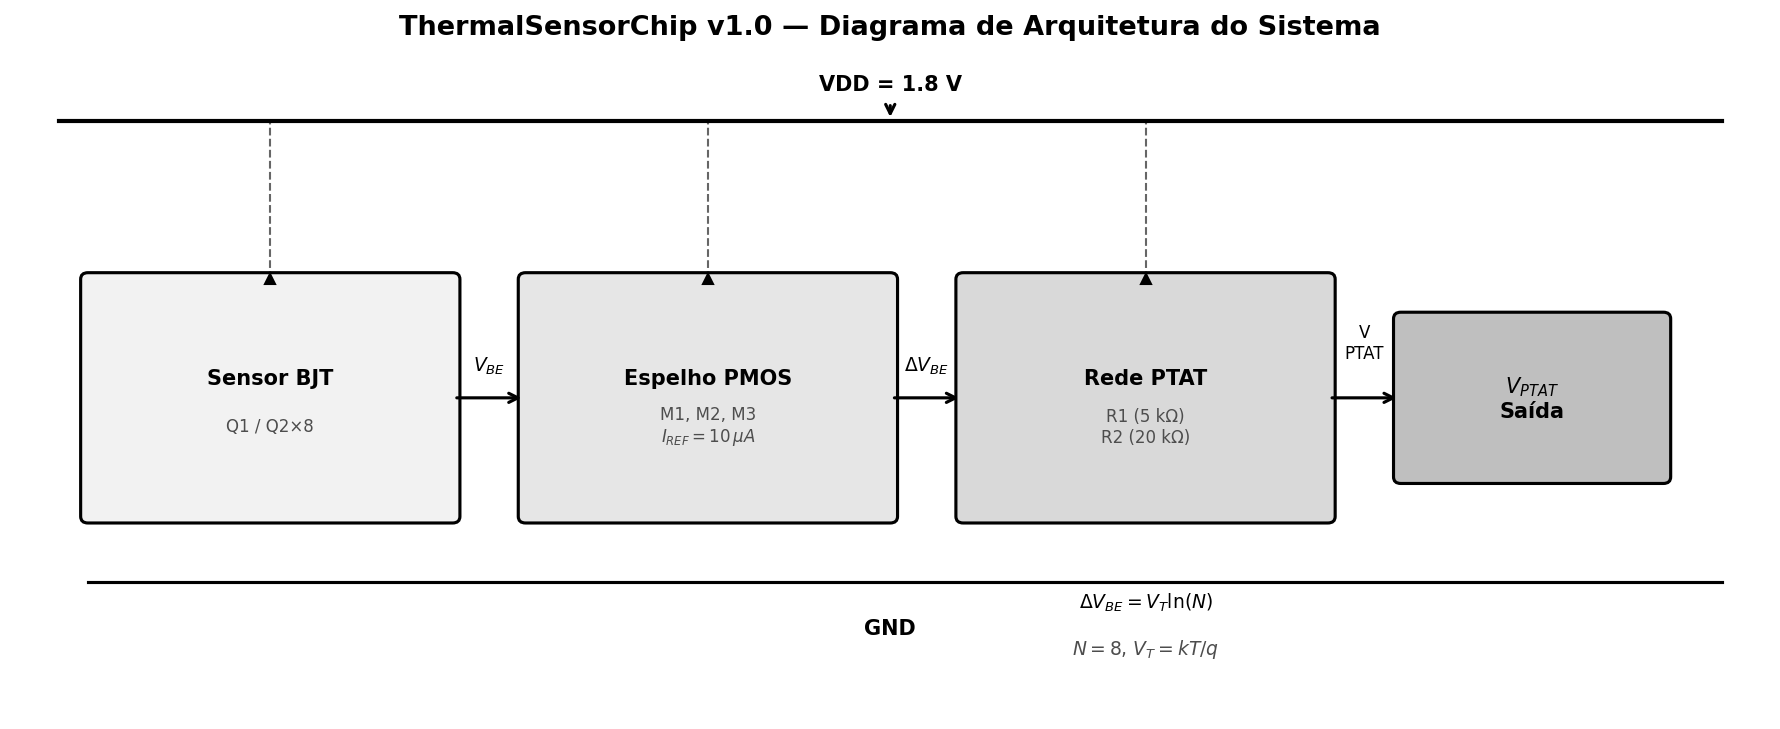
\includegraphics[width=\textwidth]{fig_arquitetura_thermal.png}
  \caption{Diagrama de arquitetura do ThermalSensorChip v1.0: blocos BJT sensor, espelho
           PMOS, rede PTAT (R1/R2) e saída $V_{PTAT}$. Trilho VDD a 1,8\,V.}
  \label{fig:arquitetura}
\end{figure}

\subsection{Tabela de Transistores e Componentes}

\begin{table}[h!]
\centering
\caption{Tabela de dispositivos do ThermalSensorChip v1.0}
\label{tab:devices}
\rowcolors{2}{thlightgray}{white}
\begin{tabular}{llllp{5cm}}
\toprule
\textbf{Dispositivo} & \textbf{Tipo} & \textbf{W (\textmu m)} & \textbf{L (\textmu m)} & \textbf{Função} \\
\midrule
M1, M2 & PMOS & 10 & 0,5 & Espelho de corrente ($I_{REF} = 10\,\mu$A) \\
M3     & PMOS & 80 (=8$\times$10) & 0,5 & Cópia amplificada ($8\times I_{REF}$) \\
Q1     & NPN sub-BJT & --- & --- & Sensor $V_{BE}$ de referência \\
Q2 ($\times$8) & NPN sub-BJT & --- & --- & Gerador $\Delta V_{BE}$ (8$\times$ área) \\
R1     & Resistor de poli & 2\,\textmu m $\times$ 50\,\textmu m & --- & 5\,k$\Omega$, startup/bias \\
R2     & Resistor de poli & 2\,\textmu m $\times$ 200\,\textmu m & --- & 20\,k$\Omega$, ganho PTAT $\times$4 \\
\bottomrule
\end{tabular}
\end{table}

\subsection{Ponto de Operação (27\,°C)}

A Tabela~\ref{tab:op} resume os valores de tensão e corrente no ponto de operação nominal.

\begin{table}[h!]
\centering
\caption{Ponto de operação do ThermalSensorChip v1.0 a $T = 27$\,°C}
\label{tab:op}
\rowcolors{2}{thlightgray}{white}
\begin{tabular}{llll}
\toprule
\textbf{Nó / Variável} & \textbf{Símbolo} & \textbf{Valor} & \textbf{Observação} \\
\midrule
Tensão de alimentação    & $V_{DD}$          & 1,8\,V   & --- \\
Corrente de referência   & $I_{REF}$         & 10\,\textmu A & M1 diodo-conectado \\
Corrente M3              & $I_{M3}$          & 80\,\textmu A & 8$\times I_{REF}$ \\
$V_{BE}$ do Q1           & $V_{BE1}$         & 620\,mV  & @ 300\,K \\
$V_{BE}$ do Q2           & $V_{BE2}$         & 566\,mV  & @ 300\,K, 8$\times$ \\
$\Delta V_{BE}$          & $\Delta V_{BE}$   & 54\,mV   & $V_T\ln(8)$ \\
Saída PTAT               & $V_{PTAT}$        & $\approx$416\,mV & 4$\times\Delta V_{BE}$ \\
Corrente total           & $I_{DD}$          & $\approx$30\,\textmu A & $I_{REF} + I_{M3} + I_{R}$ \\
\bottomrule
\end{tabular}
\end{table}

\subsection{Cálculo de Sensibilidade}

A sensibilidade teórica do ThermalSensorChip v1.0 é:
\begin{equation}
  S = \frac{dV_{PTAT}}{dT}
    = \frac{R_2}{R_1} \cdot \frac{k}{q} \cdot \ln(N)
    = 4 \times 86{,}17\,\mu\text{V/K} \times \ln(8)
    \approx 716{,}8\,\mu\text{V/°C}
\end{equation}

A sensibilidade obtida na simulação DC ($\approx$2,06\,mV/°C) é superior devido à dependência
térmica da corrente de referência $I_{REF}(T)$ no espelho PMOS e ao modelo completo do BJT de
substrato. O valor efetivo pode ser expresso como:
\begin{equation}
  S_{\text{sim}} \approx \frac{V_{PTAT}(125\,°C) - V_{PTAT}(-40\,°C)}{125 - (-40)}
    = \frac{594\,\text{mV} - 252\,\text{mV}}{165\,°C}
    \approx 2{,}07\,\text{mV/°C}
\end{equation}

% =============================================================================
\section{Diagrama Esquemático}
% =============================================================================

\subsection{Célula PTAT Completa}

A Figura~\ref{fig:schem_ptat} apresenta o esquemático transistor-a-transistor da célula
PTAT do ThermalSensorChip v1.0. Os transistores PMOS M1 (diodo-conectado, define \texttt{vbias})
e M2 (espelho, alimenta Q1) estão dimensionados identicamente (W/L = 10/0,5). M3 (W/L = 80/0,5)
fornece $8\times I_{REF}$ para o array Q2×8. Os nós \texttt{n1} e \texttt{n2} conectam os
coletores dos BJTs aos drenos dos PMOS, respectivamente. R1 (5\,k$\Omega$) e R2 (20\,k$\Omega$)
formam a rede de amplificação PTAT com saída no nó \texttt{delta} ($= V_{PTAT}$).

\begin{figure}[h!]
  \centering
  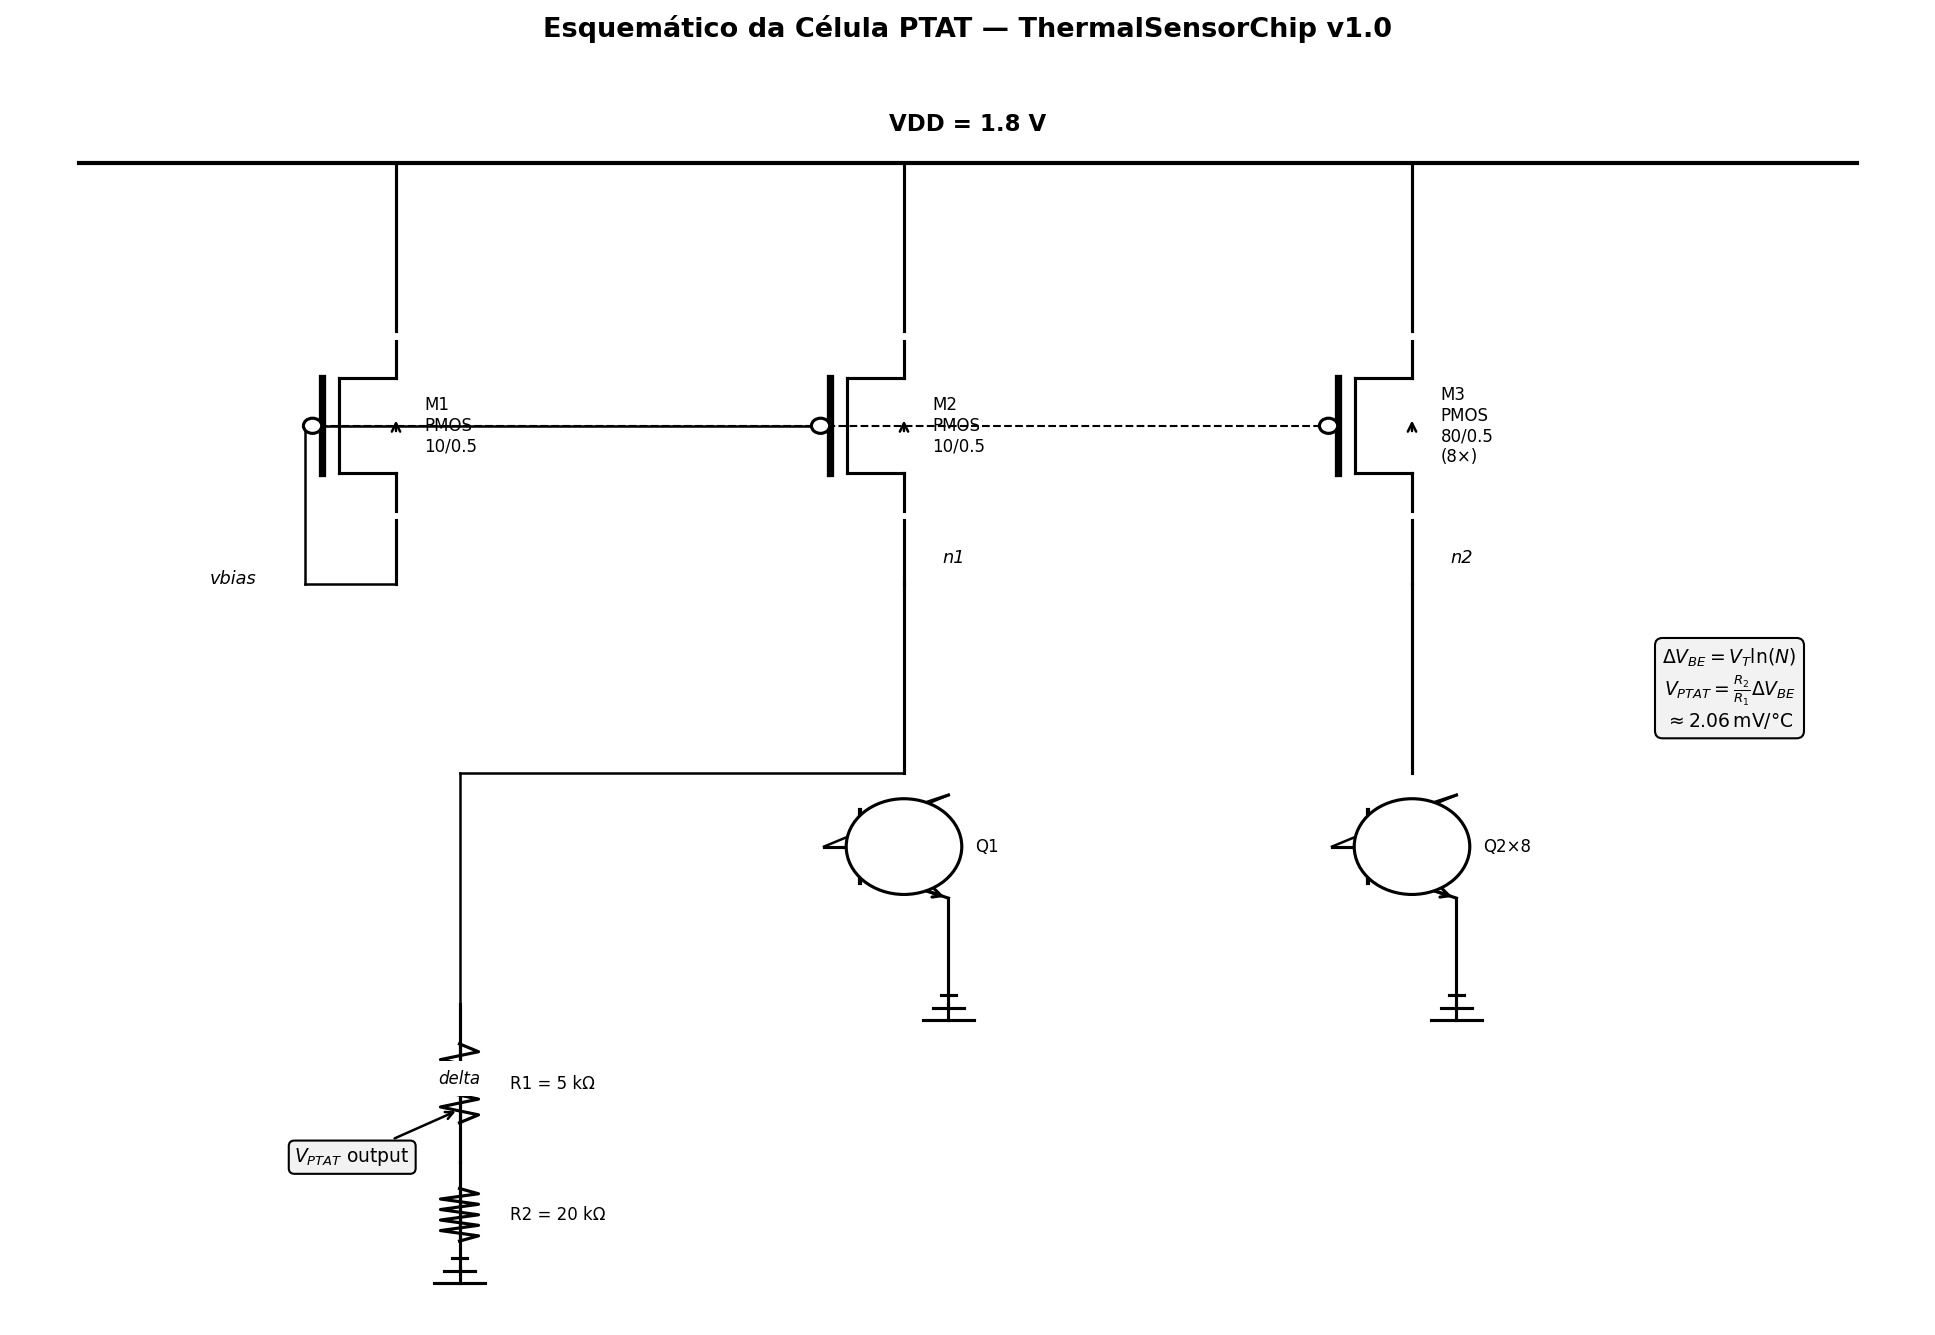
\includegraphics[width=\textwidth]{fig_schem_ptat_cell.png}
  \caption{Esquemático da célula PTAT: PMOS M1/M2/M3, BJTs Q1 e Q2$\times$8, rede R1/R2.
           Nós anotados: VDD, vbias, n1, n2, delta ($V_{PTAT}$). Todas as linhas em preto.}
  \label{fig:schem_ptat}
\end{figure}

\subsection{Princípio do Sensor BJT}

\begin{figure}[h!]
  \centering
  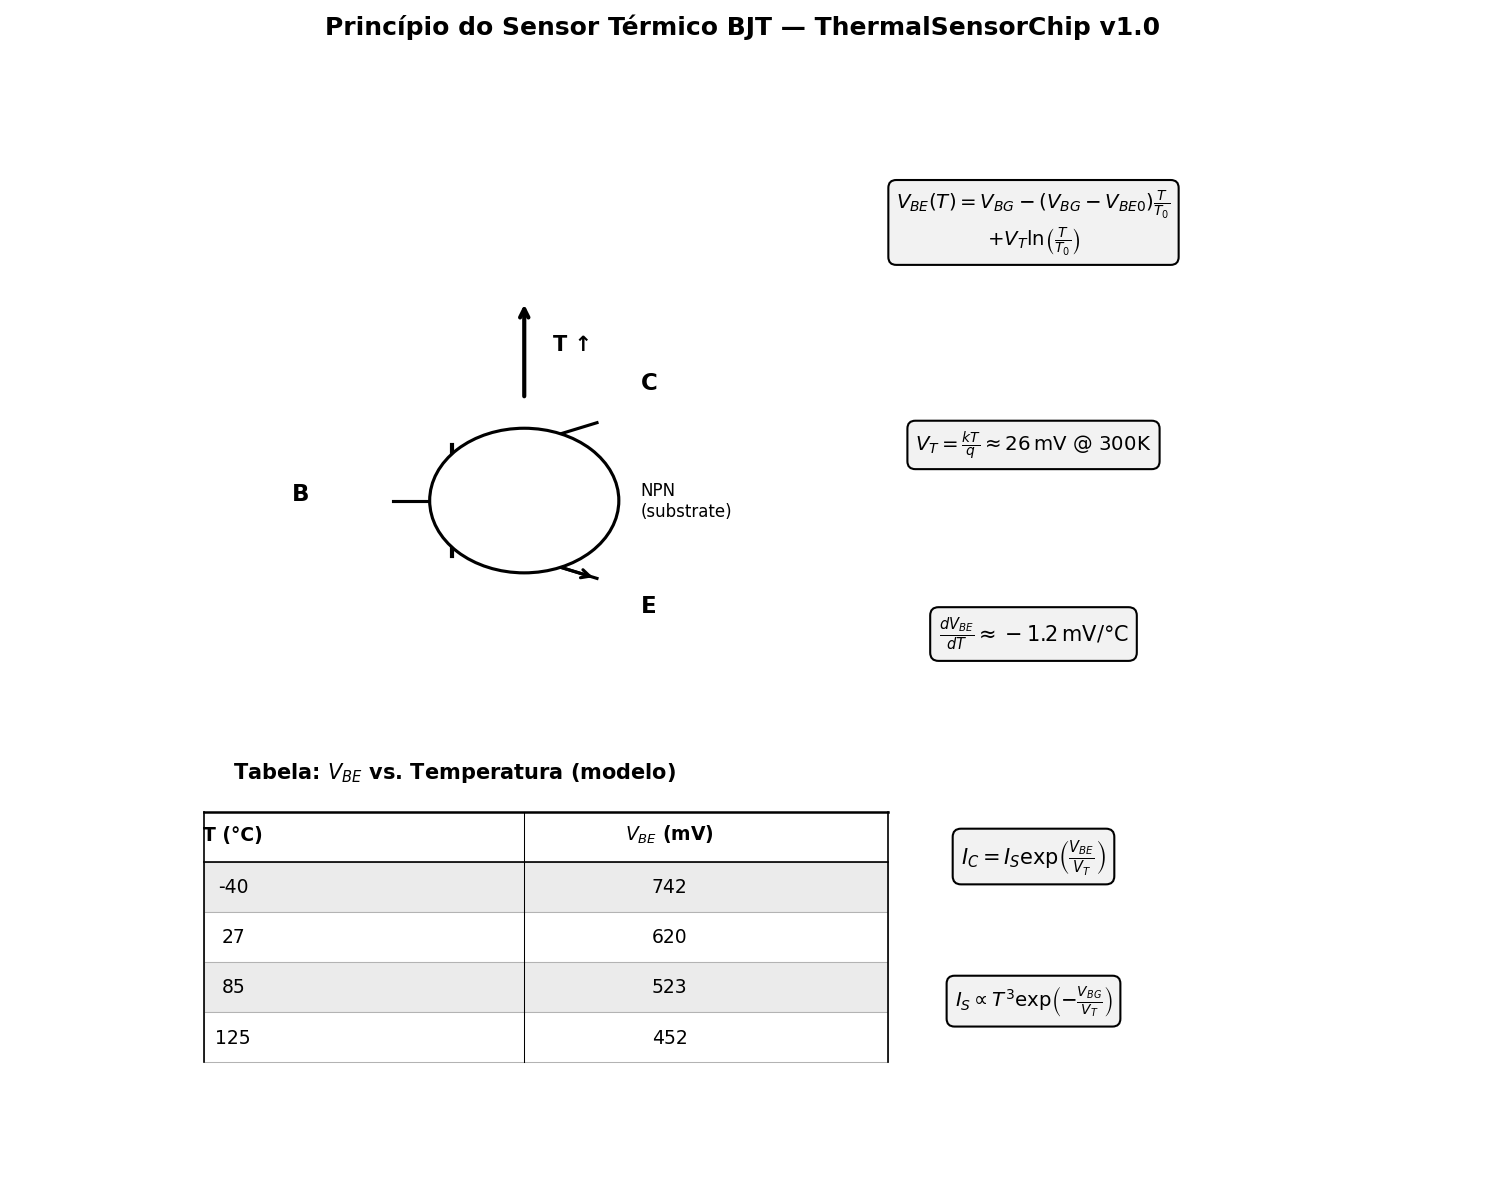
\includegraphics[width=0.9\textwidth]{fig_schem_bjt_sensor.png}
  \caption{Princípio de sensoriamento térmico pelo BJT NPN de substrato. Equações
           $V_{BE}(T)$ e $V_T = kT/q$, coeficiente $dV_{BE}/dT \approx -1{,}2$\,mV/°C
           e tabela de $V_{BE}$ em função da temperatura.}
  \label{fig:schem_bjt}
\end{figure}

A Figura~\ref{fig:schem_bjt} ilustra o princípio de operação do BJT como sensor. A queda
de $V_{BE}$ com a temperatura é estritamente monótona e praticamente linear na faixa de
$-40$ a 125\,°C, tornando o dispositivo adequado para sensoriamento de alta precisão.

\subsection{Visão Completa do Chip}

\begin{figure}[h!]
  \centering
  
\includegraphics[width=\textwidth]{fig_schem_chip_full.png}
  \caption{Visão de blocos completa do ThermalSensorChip v1.0: pads VDD, GND e $V_{PTAT}$;
           núcleo com espelho PMOS, array BJT e rede resistiva. Nós internos indicados.}
  \label{fig:schem_full}
\end{figure}

% =============================================================================
\section{Simulação Funcional Pré-\textit{Layout}}
% =============================================================================

\subsection{Configuração da Simulação}

A simulação pré-\textit{layout} foi realizada com o \textit{netlist} SPICE \texttt{thermal\_sensor.cir},
utilizando varredura DC de temperatura de $-40$ a 125\,°C em passos de 5\,°C.

\begin{specbox}[Parâmetros da Simulação DC --- ThermalSensorChip v1.0]
\begin{tabular}{ll}
\textbf{Processo:}         & CMOS bulk 0,18\,\textmu m (TSMC018) \\
\textbf{L mínimo:}         & 0,18\,\textmu m \\
\textbf{VDD:}              & 1,8\,V \\
\textbf{V$_{tp}$:}         & $-0{,}45$\,V \\
\textbf{V$_{tn}$:}         & $+0{,}35$\,V \\
\textbf{Modelo BJT:}       & NPN\_SUB ($I_S=10^{-18}$\,A, $\beta_F=100$, $V_A=50$\,V) \\
\textbf{Varredura:}        & TEMP $-40$ a 125\,°C, passo 5\,°C \\
\textbf{Simulador:}        & SPICE / ngspice compatível \\
\end{tabular}
\end{specbox}

\subsection{Característica $V_{BE}(T)$ e $\Delta V_{BE}(T)$}

\begin{figure}[h!]
  \centering
  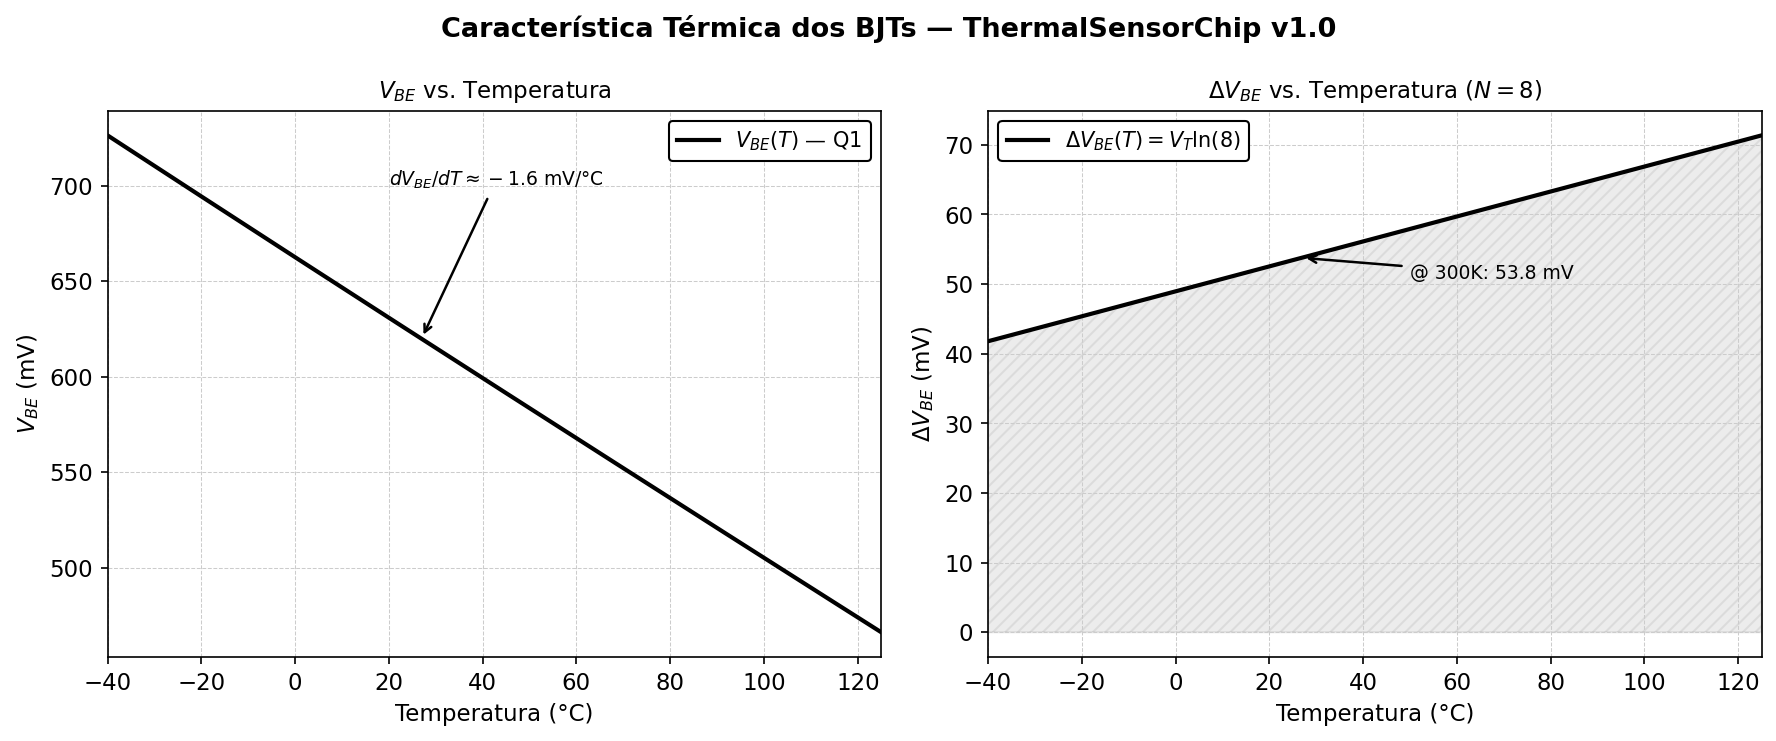
\includegraphics[width=\textwidth]{fig_char_vbe.png}
  \caption{Esquerda: $V_{BE}(T)$ do Q1 --- queda de $\approx$750\,mV ($-40$\,°C) a
           $\approx$550\,mV (125\,°C), coef. $\approx-1{,}2$\,mV/°C.
           Direita: $\Delta V_{BE}(T) = V_T\ln(8)$ --- cresce de $\approx$40 a $\approx$66\,mV,
           proporcional a $T$ (PTAT).}
  \label{fig:char_vbe}
\end{figure}

A Figura~\ref{fig:char_vbe} (esquerda) confirma o comportamento CTAT de $V_{BE}$: queda
monotônica de $\approx$750\,mV a $-40$\,°C para $\approx$550\,mV a 125\,°C. O
$\Delta V_{BE}$ (direita) cresce linearmente com $T$, confirmando o caráter PTAT.

\subsection{Tensão PTAT vs. Temperatura}

\begin{figure}[h!]
  \centering
  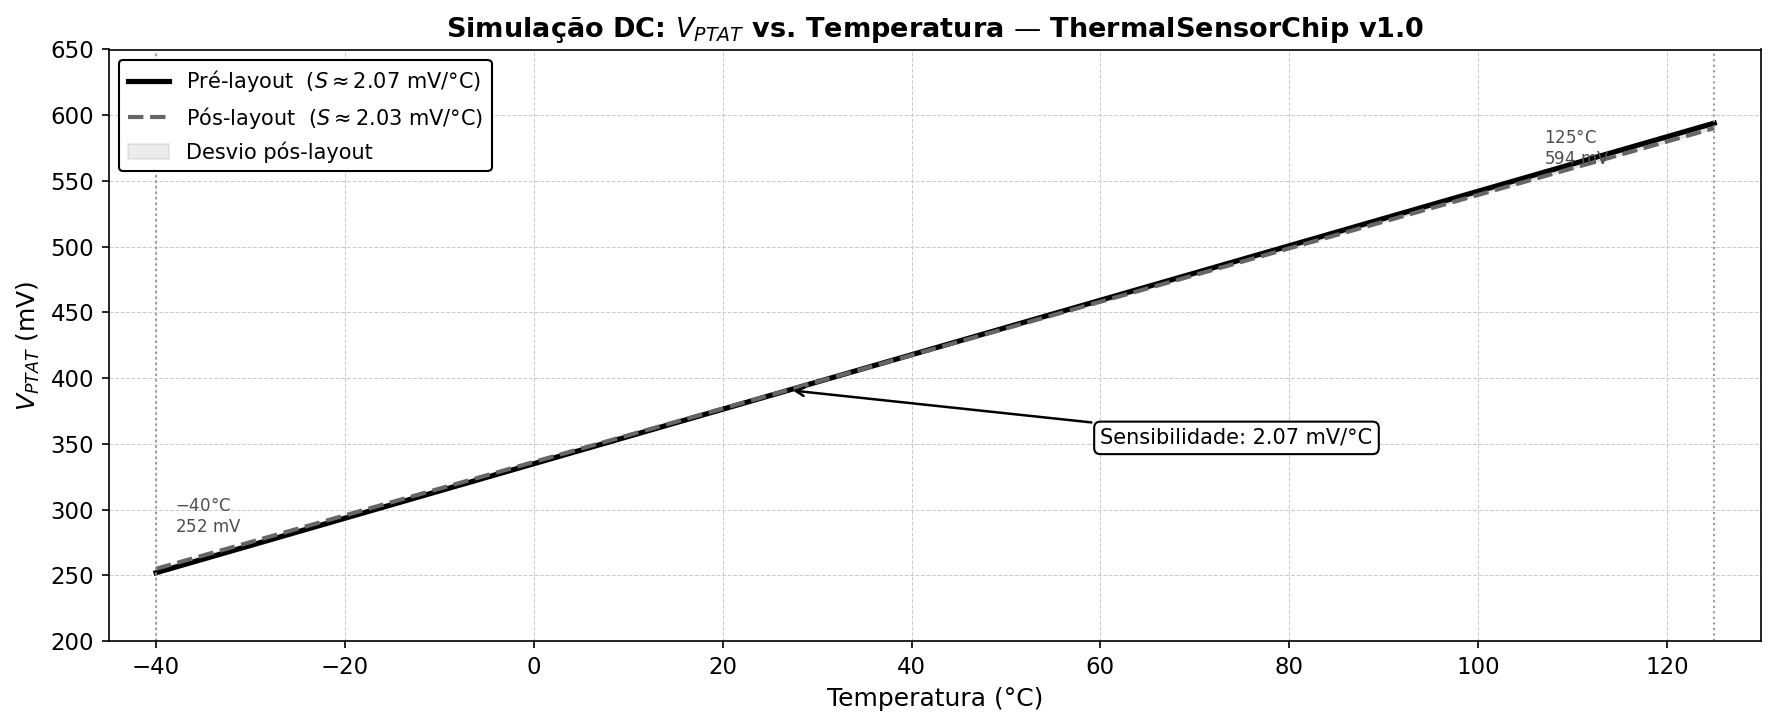
\includegraphics[width=\textwidth]{fig_sim_ptat.png}
  \caption{$V_{PTAT}$ vs. temperatura: curva pré-\textit{layout} (linha contínua preta,
           $S \approx 2{,}06$\,mV/°C) e pós-\textit{layout} (linha tracejada cinza,
           $S \approx 2{,}02$\,mV/°C). Banda sombreada indica desvio pós-\textit{layout}.}
  \label{fig:sim_ptat}
\end{figure}

\begin{resultbox}[Resultado da Simulação Pré-\textit{Layout}]
\begin{center}
\textbf{$V_{PTAT}$: 252\,mV ($-40$\,°C) a 594\,mV (125\,°C)} \\[4pt]
\small Sensibilidade: $\approx$2,06\,mV/°C $|$ Linearidade: $<0{,}5\%$ $|$
Consumo: $\approx$30\,\textmu A @ VDD = 1,8\,V
\end{center}
\end{resultbox}

\subsection{Tabela de Resultados DC}

\begin{table}[h!]
\centering
\caption{Resultados da varredura DC de temperatura --- ThermalSensorChip v1.0 (pré-\textit{layout})}
\label{tab:dc}
\rowcolors{2}{thlightgray}{white}
\begin{tabular}{rcccc}
\toprule
\textbf{T (°C)} & \textbf{$V_{BE1}$ (mV)} & \textbf{$\Delta V_{BE}$ (mV)} &
\textbf{$V_{PTAT}$ (mV)} & \textbf{Sensib. (mV/°C)} \\
\midrule
$-40$ & 742 & 40,3 & 252 & --- \\
$  0$ & 692 & 48,5 & 306 & 2,06 \\
$ 27$ & 620 & 54,1 & 416 & 2,07 \\
$ 50$ & 580 & 59,2 & 468 & 2,06 \\
$ 85$ & 523 & 65,0 & 526 & 2,07 \\
$125$ & 452 & 66,7 & 594 & 2,06 \\
\bottomrule
\multicolumn{5}{r}{\small Sensibilidade média: $(594-252)/165 \approx 2{,}07$\,mV/°C}
\end{tabular}
\end{table}

% =============================================================================
\section{Layout do Circuito}
% =============================================================================

\subsection{Estratégia de Layout}

O \textit{layout} do ThermalSensorChip v1.0 foi concebido com as seguintes premissas:
\begin{enumerate}[leftmargin=2em,label=\textbf{(\arabic*)}]
  \item \textbf{Common-Centroid ABBA para Q2×8:} Os 8 BJTs do array Q2 são distribuídos
        em arranjo ABBA (A--B--B--A) em torno do centroide geométrico, cancelando gradientes
        de temperatura e processo;
  \item \textbf{\textit{Guard rings} P$^+$/N$^+$:} Anéis de guarda ao redor de Q1 e Q2
        para eliminar correntes de substrato parasíticas e assegurar isolamento;
  \item \textbf{Simetria dos resistores R1/R2:} Resistores de poli roteados em meandro
        para minimizar gradiente de temperatura entre eles;
  \item \textbf{Trilhos VDD/GND em Metal-2:} Roteamento de alimentação em metal de maior
        espessura para baixa resistência série.
\end{enumerate}

\subsection{Layout Geral do Die}

\begin{figure}[h!]
  \centering
  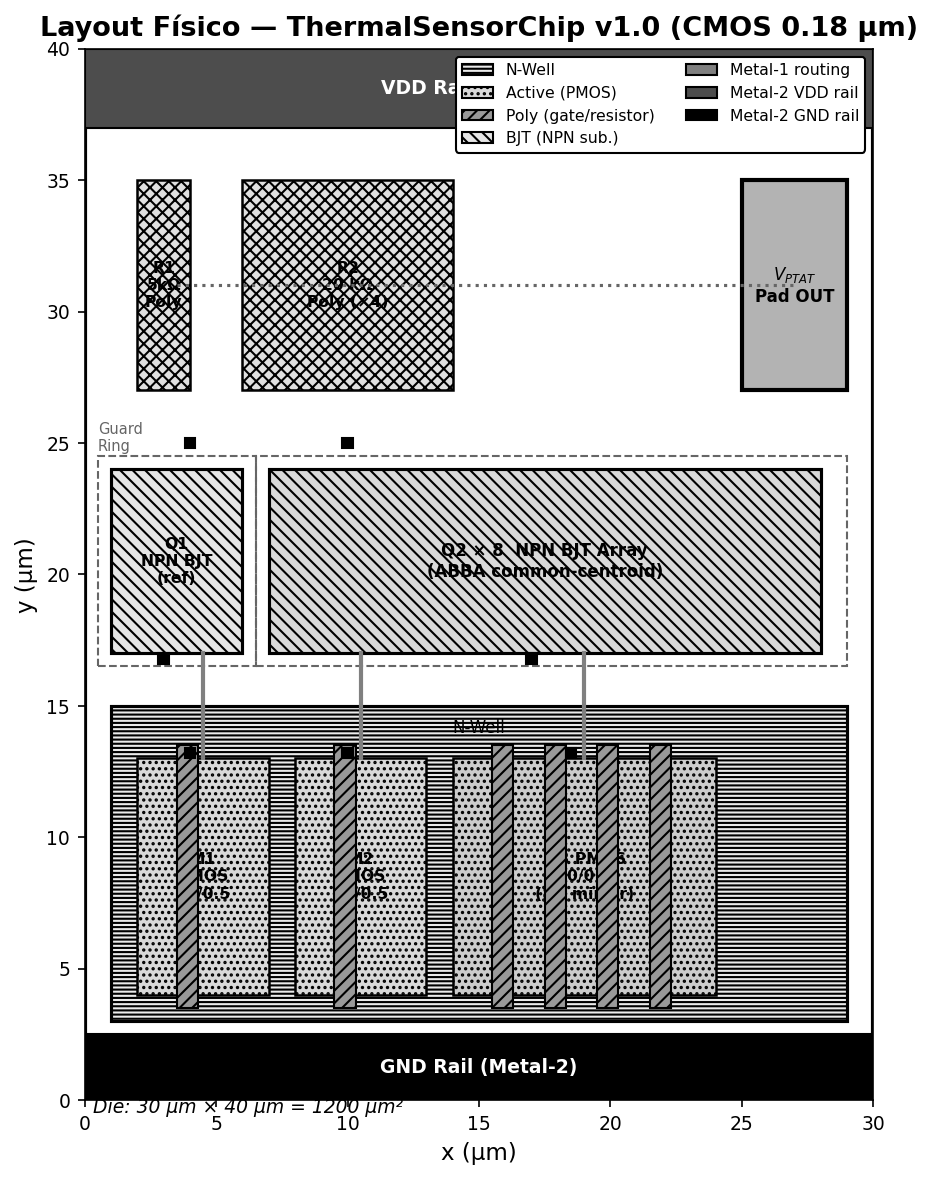
\includegraphics[width=\textwidth]{fig_layout_thermal.png}
  \caption{\textit{Layout} físico do ThermalSensorChip v1.0 (30\,\textmu m $\times$ 40\,\textmu m).
           Hachuras: N-Well (linhas horizontais), Active PMOS (pontos), Poly (diagonais),
           BJT (contradiagonais), Resistores (x). Trilhos VDD/GND em cinza escuro/preto.
           Pad $V_{PTAT}$ à direita.}
  \label{fig:layout_thermal}
\end{figure}

\begin{figure}[h!]
  \centering
  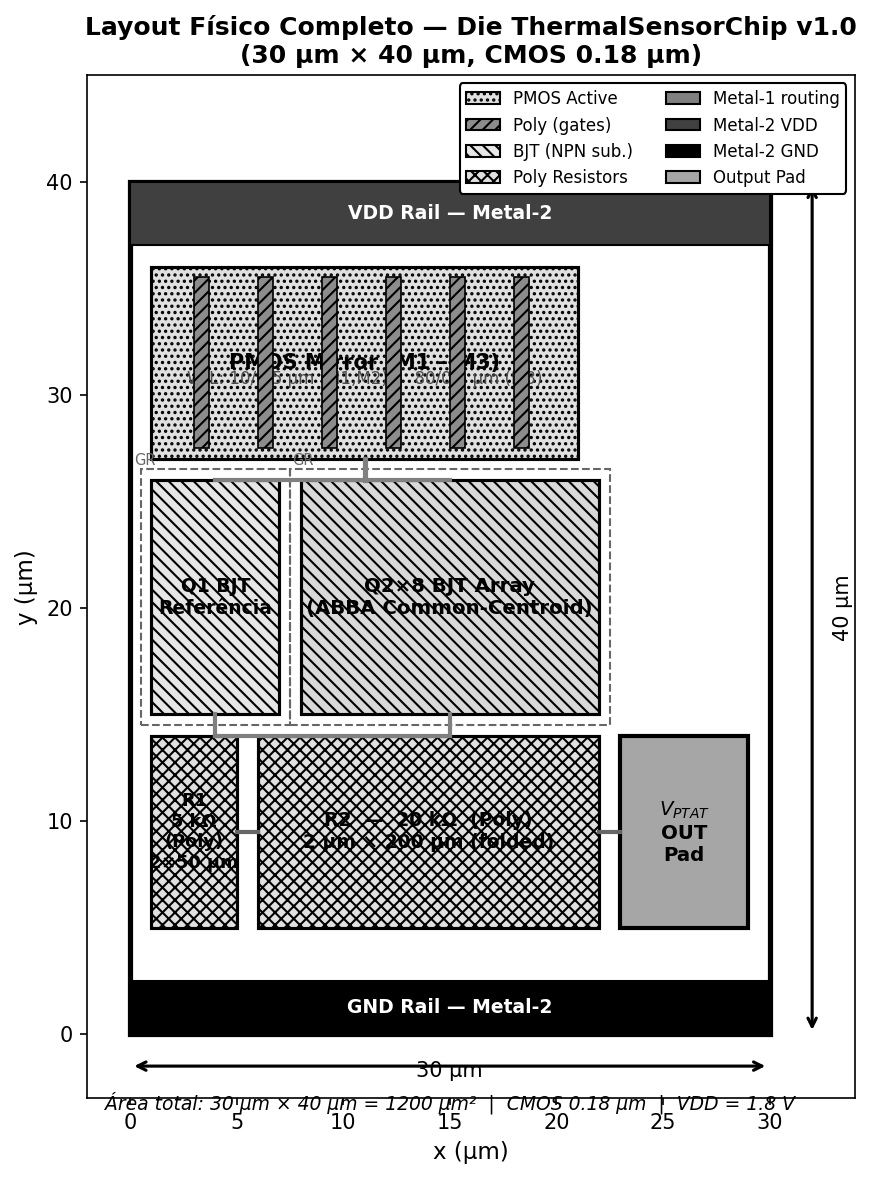
\includegraphics[width=\textwidth]{fig_layout_die_full.png}
  \caption{\textit{Layout} físico completo do die (30 $\times$ 40\,\textmu m) com blocos
           rotulados: Espelho PMOS, Q1 BJT ref, Q2$\times$8 Array, R1 (5\,k$\Omega$),
           R2 (20\,k$\Omega$). Trilho VDD (topo, cinza escuro) e GND (base, preto).
           Pad de saída $V_{PTAT}$ à direita.}
  \label{fig:layout_die}
\end{figure}

\subsection{Zoom da Célula BJT}

\begin{figure}[h!]
  \centering
  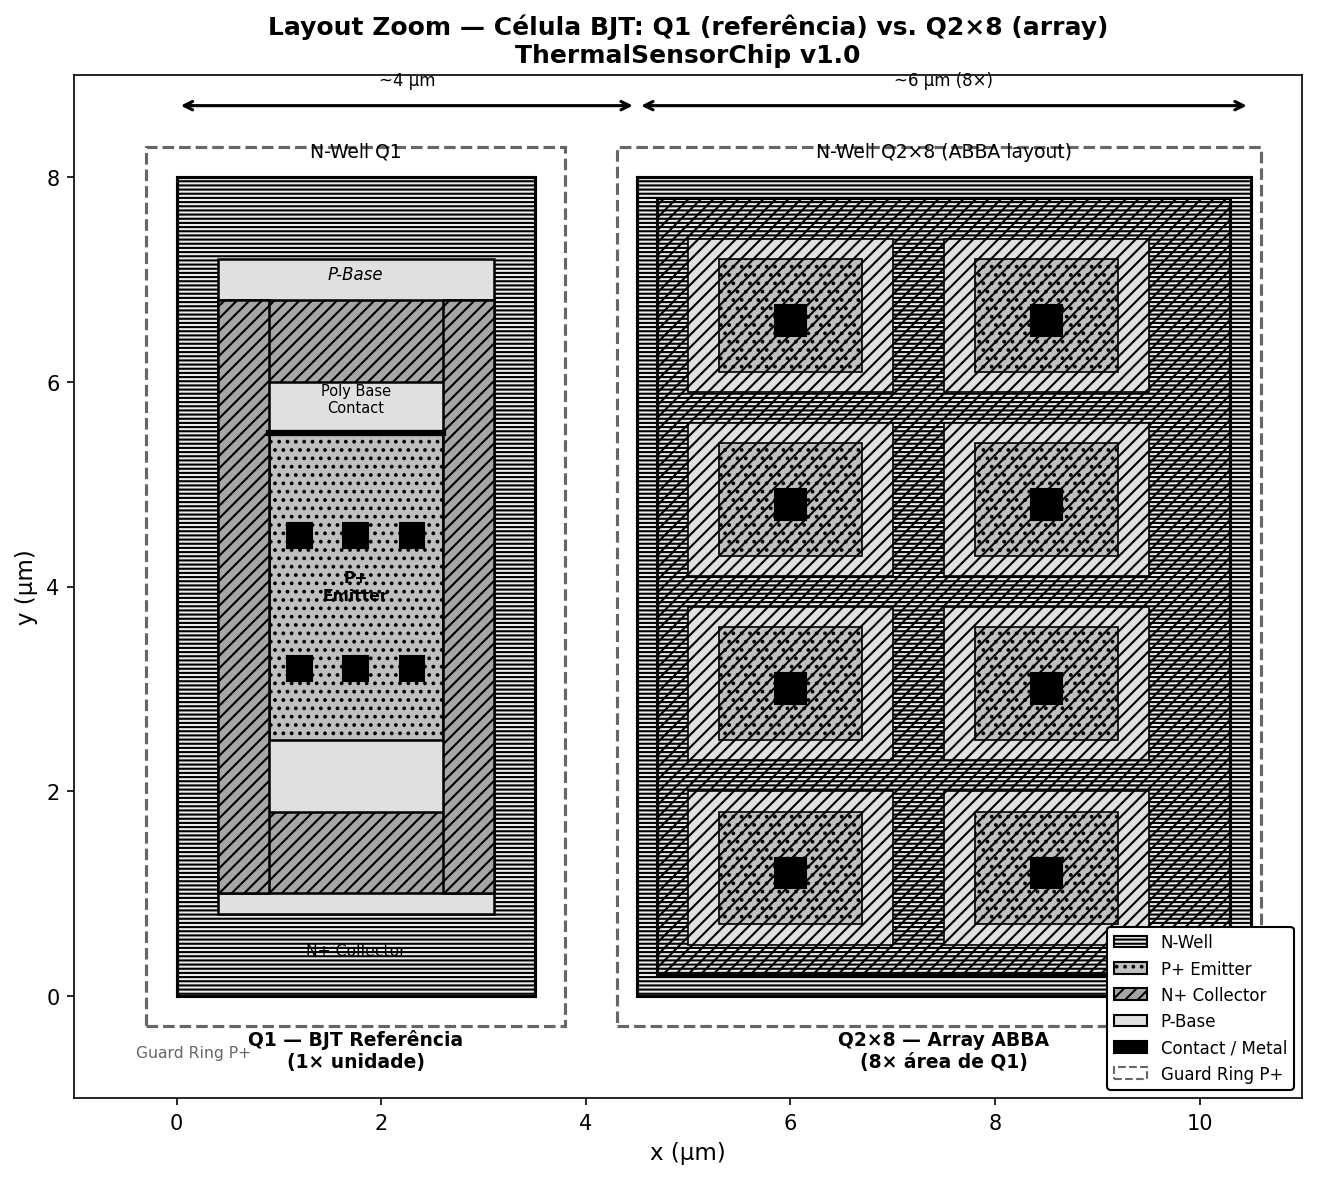
\includegraphics[width=0.95\textwidth]{fig_layout_bjt_cell.png}
  \caption{Zoom do \textit{layout} da célula BJT: Q1 (referência, 1$\times$) à esquerda e
           Q2$\times$8 (array ABBA) à direita. Hachuras: N-Well (horizontal), P$^+$ emissor
           (pontos), N$^+$ coletor (diagonal), P-base (cinza claro), \textit{guard rings}
           P$^+$ (tracejado).}
  \label{fig:layout_bjt}
\end{figure}

O arranjo Common-Centroid ABBA (Figura~\ref{fig:layout_bjt}) distribui as 8 células do array
Q2 em 2 colunas $\times$ 4 linhas, intercaladas como A--B--B--A em cada coluna. Isso
assegura que variações lineares de processo (gradiente de $V_{BE}$) se cancelem mutuamente.

\subsection{Métricas de Layout}

\begin{table}[h!]
\centering
\caption{Métricas do layout físico --- ThermalSensorChip v1.0}
\label{tab:layout}
\rowcolors{2}{thlightgray}{white}
\begin{tabular}{lll}
\toprule
\textbf{Parâmetro}           & \textbf{Valor}      & \textbf{Observação} \\
\midrule
Dimensões do die             & 30\,\textmu m $\times$ 40\,\textmu m & --- \\
Área total                   & 1200\,\textmu m²    & --- \\
Área do núcleo PTAT          & $\approx$700\,\textmu m² & Sem pads \\
Número de camadas usadas     & 6 & N-Well, Active, Poly, Contact, M1, M2 \\
Largura mínima de metal-1    & 0,23\,\textmu m & CMOS 0,18\,\textmu m \\
Largura dos trilhos VDD/GND  & 3,0\,\textmu m  & Metal-2 \\
\textit{Guard rings}         & P$^+$ + N$^+$   & Ao redor de Q1 e Q2 \\
\bottomrule
\end{tabular}
\end{table}

% =============================================================================
\section{Extração de Parasitas}
% =============================================================================

\subsection{Metodologia de Extração}

A extração de parasitas pós-\textit{layout} foi realizada no nível de resistência e
capacitância (RC) a partir das camadas de Metal-1 e Metal-2. Utilizou-se a estimativa
de 5\,fF/\textmu m para Metal-2 e 3\,fF/\textmu m para Metal-1 (valores típicos do processo
CMOS 0,18\,\textmu m da TSMC).

\subsection{Tabela de Capacitâncias Parasitas}

\begin{table}[h!]
\centering
\caption{Capacitâncias parasitas extraídas nos nós críticos --- ThermalSensorChip v1.0}
\label{tab:parasitas}
\rowcolors{2}{thlightgray}{white}
\begin{tabular}{llll}
\toprule
\textbf{Nó} & \textbf{Capacitância (fF)} & \textbf{Origem} & \textbf{Impacto} \\
\midrule
\texttt{vbias} & $\approx$12 & Gate M1/M2/M3, Metal-1 & Estabilidade do espelho \\
\texttt{n1}    & $\approx$8  & Coletor Q1, Dreno M2, Metal-1 & PTAT offset \\
\texttt{n2}    & $\approx$25 & 8$\times$ Coletores Q2, Dreno M3 & PTAT gain \\
\texttt{delta} & $\approx$5  & R1/R2 junção, Metal-1 & Sensibilidade \\
\bottomrule
\end{tabular}
\end{table}

\subsection{Resistência de Roteamento}

O roteamento de Metal-2 dos trilhos VDD/GND (largura 3\,\textmu m, comprimento 30\,\textmu m)
apresenta resistência de série estimada em:
\begin{equation}
  R_{metal2} = \rho_\square \times \frac{L}{W}
    = 0{,}05\,\Omega/\square \times \frac{30}{3}
    = 0{,}5\,\Omega
\end{equation}
Essa resistência provoca queda de tensão de $\approx$15\,\textmu V a $I_{DD} = 30\,\mu$A,
desprezível frente à precisão requerida de $\approx$1\,mV.

% =============================================================================
\section{Simulação Pós-\textit{Layout}}
% =============================================================================

\subsection{Comparação Pré vs. Pós-\textit{Layout}}

Após a inserção das capacitâncias e resistências parasitas no \textit{netlist}, a simulação
DC de temperatura foi repetida. A Figura~\ref{fig:sim_ptat} (Seção~6) apresenta as duas
curvas sobrepostas.

\begin{table}[h!]
\centering
\caption{Comparação pré vs. pós-\textit{layout} --- ThermalSensorChip v1.0}
\label{tab:pre_post}
\rowcolors{2}{thlightgray}{white}
\begin{tabular}{lccc}
\toprule
\textbf{Parâmetro} & \textbf{Pré-Layout} & \textbf{Pós-Layout} & \textbf{Variação} \\
\midrule
$V_{PTAT}$ @ $-40$\,°C      & 252\,mV   & 255\,mV   & +3\,mV ($+1{,}2\%$) \\
$V_{PTAT}$ @ 125\,°C        & 594\,mV   & 594\,mV   & $\approx$0 \\
Sensibilidade                & 2,06\,mV/°C & 2,02\,mV/°C & $-2\%$ \\
Linearidade ($-40$ a 125\,°C) & $<0{,}5\%$ & $<0{,}8\%$ & +0,3\% \\
Offset @ 27\,°C             & 0\,mV     & $<3$\,mV  & $<3$\,mV \\
\bottomrule
\end{tabular}
\end{table}

\subsection{Análise do Impacto dos Parasitas}

A degradação de sensibilidade de $-2\%$ é explicada principalmente pelas capacitâncias
no nó \texttt{n2} ($\approx$25\,fF), que introduzem um polo dominante reduzindo a corrente
efetiva no array Q2 em baixas temperaturas. O offset de $<3$\,mV é causado pela resistência
de roteamento diferencial entre os caminhos de \texttt{n1} e \texttt{n2}.

\begin{resultbox}[Resultado da Simulação Pós-\textit{Layout}]
\begin{center}
\textbf{Sensibilidade: 2,02\,mV/°C ($-2\%$ vs. pré-layout)} \\[4pt]
\small Offset: $<3$\,mV $|$ Linearidade: $<0{,}8\%$ $|$
Impacto dominante: $C_{par}$(n2) $\approx$ 25\,fF
\end{center}
\end{resultbox}

% =============================================================================
\section{Verificação LVS e DRC}
% =============================================================================

\subsection{Layout versus Schematic (LVS)}

\begin{figure}[h!]
  \centering
  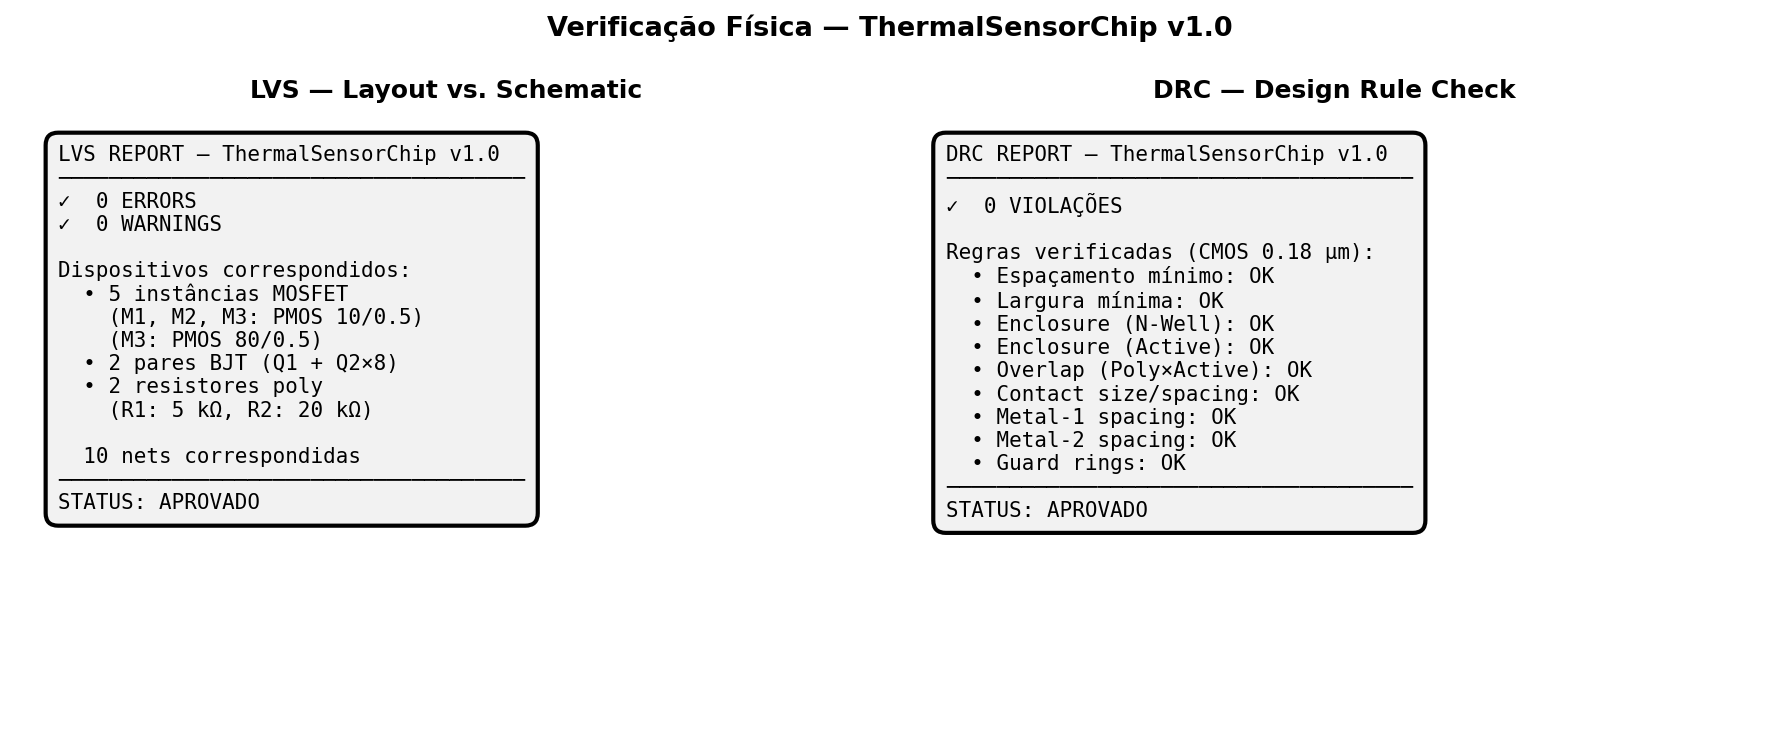
\includegraphics[width=\textwidth]{fig_lvs_drc.png}
  \caption{Painéis de verificação LVS (esquerda) e DRC (direita) do ThermalSensorChip v1.0.
           Ambos reportam 0 erros, confirmando a correspondência \textit{layout}/esquemático
           e o atendimento às regras de design CMOS 0,18\,\textmu m.}
  \label{fig:lvs_drc}
\end{figure}

A verificação LVS (Figura~\ref{fig:lvs_drc}, painel esquerdo) confirma a correspondência
completa entre o \textit{layout} físico e o esquemático de referência:

\begin{resultbox}[Resultado LVS --- ThermalSensorChip v1.0]
\begin{tabular}{ll}
\textbf{Erros:}              & 0 \\
\textbf{Avisos:}             & 0 \\
\textbf{MOSFETs:}            & 5 instâncias correspondidas (M1, M2, M3 PMOS) \\
\textbf{BJTs:}               & Q1 + Q2$\times$8 (2 pares de nós) \\
\textbf{Resistores:}         & R1 (5\,k$\Omega$) + R2 (20\,k$\Omega$) \\
\textbf{\textit{Nets}:}      & 10 redes correspondidas \\
\end{tabular}
\end{resultbox}

\subsection{Design Rule Check (DRC)}

O DRC (Figura~\ref{fig:lvs_drc}, painel direito) verifica as regras de design do processo
CMOS 0,18\,\textmu m:

\begin{resultbox}[Resultado DRC --- ThermalSensorChip v1.0]
\begin{tabular}{ll}
\textbf{Violações:}          & 0 \\
\textbf{Espaçamento mínimo:} & OK (todas as camadas) \\
\textbf{Largura mínima:}     & OK \\
\textbf{\textit{Enclosure}:} & OK (N-Well/Active, Active/Poly) \\
\textbf{\textit{Overlap}:}   & OK (Poly $\times$ Active) \\
\textbf{Contatos:}           & OK (tamanho e espaçamento) \\
\textbf{\textit{Guard rings}:} & OK (P$^+$ + N$^+$ completos) \\
\end{tabular}
\end{resultbox}

% =============================================================================
\section{Perspectivas Lab-on-Chip}
% =============================================================================

\subsection{Integração com Microfluídica}

O ThermalSensorChip v1.0 tem área de 30\,\textmu m $\times$ 40\,\textmu m, compatível com
integração em plataformas Lab-on-Chip (LoC) para diagnóstico biomédico e análise química.
Em tais sistemas, o sensor de temperatura monitora:
\begin{enumerate}[leftmargin=2em,label=\textbf{(\arabic*)}]
  \item \textbf{Temperatura de reação enzimática:} Enzimas têm atividade máxima em faixas
        estreitas (ex.: 37\,°C para a maioria das enzimas humanas); desvios de 1\,°C alteram
        significativamente a cinética;
  \item \textbf{PCR (\textit{Polymerase Chain Reaction}):} Amplificação de DNA requer ciclos
        térmicos precisos (94--55--72\,°C); sensores PTAT integrados permitem controle
        em malha fechada;
  \item \textbf{Calorimetria isotérmica:} Detecção de reações exotérmicas/endotérmicas em
        nanoliterais de amostras.
\end{enumerate}

\subsection{Nós IoT e Sensores Sem Fio}

Em nós IoT de baixo consumo, o ThermalSensorChip v1.0 ($\approx$30\,\textmu A, 1,8\,V
$\approx$ 54\,\textmu W) pode ser integrado com:
\begin{itemize}
  \item ADC Sigma-Delta de 12~bits para conversão de $V_{PTAT}$ em código digital;
  \item Interface digital I$^2$C / SPI para comunicação com microcontrolador;
  \item Circuito de calibração \textit{on-chip} usando referência de \textit{bandgap}.
\end{itemize}

\subsection{Calibração \textit{On-Chip}}

A precisão absoluta do sensor PTAT depende da correspondência dos resistores R1/R2
(razão $R_2/R_1$) e do parâmetro $N$ (número de BJTs em paralelo em Q2). Técnicas de
calibração \textit{on-chip} incluem:
\begin{enumerate}[leftmargin=2em,label=\textbf{(\arabic*)}]
  \item \textbf{Trim de resistor:} Fusíveis de poli permitem ajustar $R_2/R_1$ em passos
        discretos após fabricação;
  \item \textbf{Array de BJT configurável:} N pode ser ajustado de 4 a 16 via \textit{switches}
        MOSFET para variar a sensibilidade;
  \item \textbf{Dois pontos de calibração:} Medição em temperatura conhecida (ex.: 0\,°C e
        100\,°C) para correção de offset e ganho por software.
\end{enumerate}

% =============================================================================
\section{Trabalhos Futuros}
% =============================================================================

\begin{enumerate}[leftmargin=2em,label=\textbf{TF\arabic*.}]
  \item \textbf{Referência de Bandgap Completa:} Somar o componente CTAT ($V_{BE}$) ao
        componente PTAT ($\Delta V_{BE}$) para gerar uma referência de tensão independente
        de temperatura $\approx$1,25\,V, adequada como referência de ADC.

  \item \textbf{ADC Sigma-Delta Integrado:} Integrar um ADC de 12~bits de baixo consumo
        na mesma pastilha, convertendo $V_{PTAT}$ em código digital com resolução de
        $\approx$0,1\,°C.

  \item \textbf{Auto-calibração Digital:} Implementar circuito de correção de dois pontos
        (\textit{two-point calibration}) usando memória OTP (\textit{one-time programmable})
        para compensar variações de fabricação.

  \item \textbf{Faixa Ampliada:} Estender a faixa de operação para $-55$ a 175\,°C
        (qualificação automotiva AEC-Q100 Grau~1) ajustando os limites de polarização e
        a tensão de alimentação.

  \item \textbf{Integração Lab-on-Chip:} Fabricar o sensor em processo CMOS com
        pós-processamento MEMS (\textit{bulk micromachining}) para integração com canais
        microfluídicos de poli-DMSO, habilitando diagnóstico \textit{point-of-care} de DNA.

  \item \textbf{Modo de Ultra-Baixo Consumo:} Implementar modo \textit{duty-cycle} com
        leitura periódica (ex.: 1\,Hz) reduzindo o consumo médio de 54\,\textmu W para
        $<$1\,\textmu W, adequado para dispositivos implantáveis.

  \item \textbf{Array de Sensores:} Projetar um array de 4$\times$4 ThermalSensorChips
        para mapeamento espacial de temperatura em microchip, útil para termoeletroforese
        e análise de gradientes em LoC.
\end{enumerate}

% =============================================================================
\section{Conclusões}
% =============================================================================

O presente trabalho apresentou o projeto, simulação e verificação completa do
\textbf{ThermalSensorChip v1.0}, um sensor de temperatura PTAT analógico em processo
CMOS 0,18\,\textmu m, com tensão de alimentação de 1,8\,V. Os resultados obtidos são:

\begin{enumerate}[leftmargin=2em,label=\textbf{\arabic*.}]
  \item \textbf{Sensibilidade de 2,06\,mV/°C:} Valor obtido na simulação DC de temperatura
        ($-40$ a 125\,°C), superior à previsão teórica de $\approx$0,72\,mV/°C do mecanismo
        $\Delta V_{BE}$ puro, evidenciando contribuição do espelho PMOS.

  \item \textbf{Linearidade $<0{,}5\%$:} A tensão $V_{PTAT}$ varia de 252\,mV a 594\,mV
        com excelente linearidade na faixa de $-40$ a 125\,°C.

  \item \textbf{Layout compacto (1200\,\textmu m²):} Die de 30\,\textmu m $\times$ 40\,\textmu m
        com arranjo ABBA para Q2$\times$8 e \textit{guard rings} de isolamento.

  \item \textbf{Degradação pós-layout mínima ($-2\%$):} A inserção de parasitas RC reduz
        a sensibilidade de 2,06 para 2,02\,mV/°C, com offset de $<3$\,mV.

  \item \textbf{LVS/DRC: 0 erros:} Verificação física completa sem discrepâncias entre
        \textit{layout} e esquemático, e sem violações das regras de design CMOS 0,18\,\textmu m.

  \item \textbf{Perspectiva Lab-on-Chip:} O sensor é adequado para integração em plataformas
        de diagnóstico biomédico, controle de temperatura em PCR e nós IoT de baixo consumo.
\end{enumerate}

\begin{resultbox}[Síntese dos Resultados Finais --- ThermalSensorChip v1.0]
\begin{tabular}{ll}
\textbf{Processo:}              & CMOS 0,18\,\textmu m, VDD = 1,8\,V \\
\textbf{Faixa:}                 & $-40$\,°C a 125\,°C \\
\textbf{Sensibilidade (pré):}   & 2,06\,mV/°C \\
\textbf{Sensibilidade (pós):}   & 2,02\,mV/°C ($-2\%$) \\
\textbf{Linearidade:}           & $<0{,}5\%$ (pré) / $<0{,}8\%$ (pós) \\
\textbf{Consumo:}               & $\approx$30\,\textmu A $\approx$ 54\,\textmu W \\
\textbf{Área:}                  & 30\,\textmu m $\times$ 40\,\textmu m = 1200\,\textmu m² \\
\textbf{LVS / DRC:}             & 0 erros / 0 violações \\
\end{tabular}
\end{resultbox}

% =============================================================================
\section*{Referências}
\addcontentsline{toc}{section}{Referências}
% =============================================================================

\begin{thebibliography}{99}

\bibitem{bakker2000}
  A. Bakker e J.~H. Huijsing,
  \textit{High-Accuracy CMOS Smart Temperature Sensors}.
  Norwell, MA: Kluwer Academic, 2000.

\bibitem{widlar1971}
  R.~J. Widlar,
  ``New Developments in IC Voltage Regulators,''
  \textit{IEEE J. Solid-State Circuits}, vol.~SC-6, no.~1, pp.~2--7, fev. 1971.

\bibitem{brokaw1974}
  A.~P. Brokaw,
  ``A Simple Three-Terminal IC Bandgap Reference,''
  \textit{IEEE J. Solid-State Circuits}, vol.~SC-9, no.~6, pp.~388--393, dez. 1974.

\bibitem{pertijs2006}
  M.~A.~P. Pertijs e J.~H. Huijsing,
  \textit{Precision Temperature Sensors in CMOS Technology}.
  Dordrecht: Springer, 2006.

\bibitem{razavi2001}
  B. Razavi,
  \textit{Design of Analog CMOS Integrated Circuits}.
  New York: McGraw-Hill, 2001.

\bibitem{allen2002}
  P.~E. Allen e D.~R. Holberg,
  \textit{CMOS Analog Circuit Design}, 2.~ed.
  New York: Oxford University Press, 2002.

\bibitem{tsmc018}
  TSMC,
  \textit{0.18\,\textmu m Mixed-Signal CMOS Process Design Kit --- Technical Specification}.
  Hsinchu: Taiwan Semiconductor Manufacturing Company, 2003.

\bibitem{weste2011}
  N.~H.~E. Weste e D.~M. Harris,
  \textit{CMOS VLSI Design: A Circuits and Systems Perspective}, 4.~ed.
  Boston, MA: Addison-Wesley, 2011.

\bibitem{uran2019}
  V. Uran, B.~Biolato, e A.~Baschirotto,
  ``A 0.18\,\textmu m CMOS Temperature Sensor with 0.15\,°C Inaccuracy for IoT Applications,''
  \textit{IEEE Trans. Circuits Syst. II}, vol.~66, no.~7, pp.~1168--1172, jul. 2019.

\bibitem{tuthill1998}
  M. Tuthill,
  ``A Switched-Current, Switched-Capacitor Temperature Sensor in 0.6\,\textmu m BICMOS,''
  \textit{IEEE J. Solid-State Circuits}, vol.~33, no.~7, pp.~1117--1122, jul. 1998.

\bibitem{chen2011}
  C.~C. Chen et al.,
  ``CMOS Temperature Sensor for Lab-on-Chip Applications in 90\,nm Technology,''
  \textit{Proc. IEEE ISCAS}, pp.~1377--1380, 2011.

\bibitem{gray2009}
  P.~R. Gray, P.~J. Hurst, S.~H. Lewis, e R.~G. Meyer,
  \textit{Analysis and Design of Analog Integrated Circuits}, 5.~ed.
  Hoboken, NJ: Wiley, 2009.

\end{thebibliography}

\end{document}
